\documentclass[12pt,addpoints]{exam}
\usepackage{amsmath, amssymb, amsthm, enumerate, graphicx}
\usepackage[usenames,dvipsnames]{color}
\usepackage{todonotes}
\usepackage{bm}
\usepackage[colorlinks=true,urlcolor=blue]{hyperref}
\usepackage{geometry}
\geometry{margin=1in}
\usepackage{float}
\usepackage{graphics}
\setlength{\marginparwidth}{2.15cm}
\usepackage{booktabs}
\usepackage{enumitem}
\usepackage{epsfig}
\usepackage{setspace}
\usepackage{parskip}
\usepackage[normalem]{ulem}
\usepackage{tikz}
\usetikzlibrary{positioning, arrows, automata}
\usepackage{pgfplots}
\usepgfplotslibrary{fillbetween}
\usepackage[font=scriptsize]{subcaption}
\usepackage{float}
\usepackage{algorithmicx}
\usepackage[noend]{algpseudocode}
\usepackage{environ}
\usepackage{bbm}
\usepackage{graphicx}
\usepackage{titling}
\usepackage{url}
\usepackage{xcolor}
\usepackage{lipsum}
\usepackage{lastpage}
\usepackage[colorlinks=true,urlcolor=blue]{hyperref}
\usepackage{multicol}
\usepackage{tabularx}
\usepackage{comment}
\usepackage{amsmath}
\usepackage{nicefrac}
\usepackage[tableposition=top]{caption}
\usepackage[many]{tcolorbox}
\usepackage{colortbl}
\usepackage{array}
\usepackage{multirow}
\usepackage{listings}
\usepackage{color}
\usepackage{adjustbox}
\usepackage{wasysym} % For \CIRCLE
\usepackage{cancel} % For \xcancel

\pgfplotsset{compat=1.16}


\definecolor{dkgreen}{rgb}{0,0.6,0}
\definecolor{gray}{rgb}{0.5,0.5,0.5}
\definecolor{mauve}{rgb}{0.58,0,0.82}

\lstset{frame=tb,
  language=Python,
  aboveskip=3mm,
  belowskip=3mm,
  showstringspaces=false,
  columns=flexible,
  basicstyle={\small\ttfamily},
  numbers=none,
  numberstyle=\tiny\color{gray},
  keywordstyle=\color{blue},
  commentstyle=\color{dkgreen},
  stringstyle=\color{mauve},
  breaklines=true,
  breakatwhitespace=true,
  tabsize=3
}


\newcommand{\class}{10-301/601 Machine Learning}
\newcommand{\term}{Spring 2023}
\newcommand{\examnum}{Exam 2}
\newcommand{\examdate}{11/09/2023}
\newcommand{\timelimit}{120 minutes}
\newcommand{\argmax}{\operatornamewithlimits{arg\,max}}
\newcommand{\argmin}{\operatornamewithlimits{arg\,min}}

% Instead of lines, use blank space.
%\renewcommand{\fillwithlines}[1]{\vspace{#1}}

\def\x{\mathbf x}
\def\y{\mathbf y}
\def\w{\mathbf w}
\def\v{\mathbf v}
\def\E{\mathbb E}
\def\V{\mathbb V}
\def\a{\mathbf a}
\def\z{\mathbf z}

\newcommand\MyBox[1]{%
  \fbox{\parbox[c][1.7cm][c]{1.7cm}{\centering #1}}%
}
\newcommand\MyVBox[1]{%
  \parbox[c][1.7cm][c]{2.5cm}{\centering\bfseries #1}%
}  
\newcommand\MyHBox[2][\dimexpr1.7cm+2\fboxsep\relax]{%
  \parbox[c][1cm][c]{#1}{\centering\bfseries #2}%
}  
\newcommand\MyTBox[3]{
  \MyVBox{#1}\MyBox{#2}
  \MyBox{#3}\par
}


\newcommand{\pts}[1]{(#1 points)}

% SOLUTION environment
\newenvironment{soln}{\leavevmode\color{red}\ignorespaces }{}

% QUESTION AUTHORS environment
\newenvironment{qauthor}{\leavevmode\color{blue}\ignorespaces }{}

% Question tester comment environment
\newenvironment{qtester}{\leavevmode\color{green}\ignorespaces}{}

% TO ONLY SHOW HOMEWORK QUESTIONS, include following (else comment out):
   % \RenewEnviron{soln}{}
   \RenewEnviron{qauthor}{}
  \RenewEnviron{qtester}{}

\newcommand{\norm}[1]{\lVert #1 \rVert}
\newcommand{\st}{\mathrm{s.t.}}

\makeatletter
\newcommand{\removelatexerror}{\let\@latex@error\@gobble}
\makeatother

\setlength\linefillheight{.35in}

%%%%%%%%%%%%%%%%%%%%%%%%%%%%%%%%%%%%%%%%%%
% Custom commands                        %
%%%%%%%%%%%%%%%%%%%%%%%%%%%%%%%%%%%%%%%%%%

% First argument is width, second argument is label.
\newcommand{\blankforFITB}[2]{\underline{\hspace{#1}#2\hspace{#1}}}

\newcommand{\vc}[1]{\boldsymbol{#1}}

\newcommand{\fpartial}[2]{\frac{\partial #1}{\partial #2}}
\newcommand{\adj}[1]{\frac{\partial J}{\partial #1}}
\newcommand{\chain}[2]{\adj{#2} = \adj{#1}\frac{\partial #1}{\partial #2}}

% mathcal
\newcommand{\Ac}{\mathcal{A}}
\newcommand{\Bc}{\mathcal{B}}
\newcommand{\Cc}{\mathcal{C}}
\newcommand{\Dc}{\mathcal{D}}
\newcommand{\Ec}{\mathcal{E}}
\newcommand{\Fc}{\mathcal{F}}
\newcommand{\Gc}{\mathcal{G}}
\newcommand{\Hc}{\mathcal{H}}
\newcommand{\Ic}{\mathcal{I}}
\newcommand{\Jc}{\mathcal{J}}
\newcommand{\Kc}{\mathcal{K}}
\newcommand{\Lc}{\mathcal{L}}
\newcommand{\Mc}{\mathcal{M}}
\newcommand{\Nc}{\mathcal{N}}
\newcommand{\Oc}{\mathcal{O}}
\newcommand{\Pc}{\mathcal{P}}
\newcommand{\Qc}{\mathcal{Q}}
\newcommand{\Rc}{\mathcal{R}}
\newcommand{\Sc}{\mathcal{S}}
\newcommand{\Tc}{\mathcal{T}}
\newcommand{\Uc}{\mathcal{U}}
\newcommand{\Vc}{\mathcal{V}}
\newcommand{\Wc}{\mathcal{W}}
\newcommand{\Xc}{\mathcal{X}}
\newcommand{\Yc}{\mathcal{Y}}
\newcommand{\Zc}{\mathcal{Z}}

% mathbb
\newcommand{\Ab}{\mathbb{A}}
\newcommand{\Bb}{\mathbb{B}}
\newcommand{\Cb}{\mathbb{C}}
\newcommand{\Db}{\mathbb{D}}
\newcommand{\Eb}{\mathbb{E}}
\newcommand{\Fb}{\mathbb{F}}
\newcommand{\Gb}{\mathbb{G}}
\newcommand{\Hb}{\mathbb{H}}
\newcommand{\Ib}{\mathbb{I}}
\newcommand{\Jb}{\mathbb{J}}
\newcommand{\Kb}{\mathbb{K}}
\newcommand{\Lb}{\mathbb{L}}
\newcommand{\Mb}{\mathbb{M}}
\newcommand{\Nb}{\mathbb{N}}
\newcommand{\Ob}{\mathbb{O}}
\newcommand{\Pb}{\mathbb{P}}
\newcommand{\Qb}{\mathbb{Q}}
\newcommand{\Rb}{\mathbb{R}}
\newcommand{\Sb}{\mathbb{S}}
\newcommand{\Tb}{\mathbb{T}}
\newcommand{\Ub}{\mathbb{U}}
\newcommand{\Vb}{\mathbb{V}}
\newcommand{\Wb}{\mathbb{W}}
\newcommand{\Xb}{\mathbb{X}}
\newcommand{\Yb}{\mathbb{Y}}
\newcommand{\Zb}{\mathbb{Z}}

% mathbf lowercase
\newcommand{\av}{\mathbf{a}}
\newcommand{\bv}{\mathbf{b}}
\newcommand{\cv}{\mathbf{c}}
\newcommand{\dv}{\mathbf{d}}
\newcommand{\ev}{\mathbf{e}}
\newcommand{\fv}{\mathbf{f}}
\newcommand{\gv}{\mathbf{g}}
\newcommand{\hv}{\mathbf{h}}
\newcommand{\iv}{\mathbf{i}}
\newcommand{\jv}{\mathbf{j}}
\newcommand{\kv}{\mathbf{k}}
\newcommand{\lv}{\mathbf{l}}
\newcommand{\mv}{\mathbf{m}}
\newcommand{\nv}{\mathbf{n}}
\newcommand{\ov}{\mathbf{o}}
\newcommand{\pv}{\mathbf{p}}
\newcommand{\qv}{\mathbf{q}}
\newcommand{\rv}{\mathbf{r}}
\newcommand{\sv}{\mathbf{s}}
\newcommand{\tv}{\mathbf{t}}
\newcommand{\uv}{\mathbf{u}}
\newcommand{\vv}{\mathbf{v}}
\newcommand{\wv}{\mathbf{w}}
\newcommand{\xv}{\mathbf{x}}
\newcommand{\yv}{\mathbf{y}}
\newcommand{\zv}{\mathbf{z}}

% mathbf uppercase
\newcommand{\Av}{\mathbf{A}}
\newcommand{\Bv}{\mathbf{B}}
\newcommand{\Cv}{\mathbf{C}}
\newcommand{\Dv}{\mathbf{D}}
\newcommand{\Ev}{\mathbf{E}}
\newcommand{\Fv}{\mathbf{F}}
\newcommand{\Gv}{\mathbf{G}}
\newcommand{\Hv}{\mathbf{H}}
\newcommand{\Iv}{\mathbf{I}}
\newcommand{\Jv}{\mathbf{J}}
\newcommand{\Kv}{\mathbf{K}}
\newcommand{\Lv}{\mathbf{L}}
\newcommand{\Mv}{\mathbf{M}}
\newcommand{\Nv}{\mathbf{N}}
\newcommand{\Ov}{\mathbf{O}}
\newcommand{\Pv}{\mathbf{P}}
\newcommand{\Qv}{\mathbf{Q}}
\newcommand{\Rv}{\mathbf{R}}
\newcommand{\Sv}{\mathbf{S}}
\newcommand{\Tv}{\mathbf{T}}
\newcommand{\Uv}{\mathbf{U}}
\newcommand{\Vv}{\mathbf{V}}
\newcommand{\Wv}{\mathbf{W}}
\newcommand{\Xv}{\mathbf{X}}
\newcommand{\Yv}{\mathbf{Y}}
\newcommand{\Zv}{\mathbf{Z}}

% bold greek lowercase
\newcommand{\alphav     }{\boldsymbol \alpha     }
\newcommand{\betav      }{\boldsymbol \beta      }
\newcommand{\gammav     }{\boldsymbol \gamma     }
\newcommand{\deltav     }{\boldsymbol \delta     }
\newcommand{\epsilonv   }{\boldsymbol \epsilon   }
\newcommand{\varepsilonv}{\boldsymbol \varepsilon}
\newcommand{\zetav      }{\boldsymbol \zeta      }
\newcommand{\etav       }{\boldsymbol \eta       }
\newcommand{\thetav     }{\boldsymbol \theta     }
\newcommand{\varthetav  }{\boldsymbol \vartheta  }
\newcommand{\iotav      }{\boldsymbol \iota      }
\newcommand{\kappav     }{\boldsymbol \kappa     }
\newcommand{\varkappav  }{\boldsymbol \varkappa  }
\newcommand{\lambdav    }{\boldsymbol \lambda    }
\newcommand{\muv        }{\boldsymbol \mu        }
\newcommand{\nuv        }{\boldsymbol \nu        }
\newcommand{\xiv        }{\boldsymbol \xi        }
\newcommand{\omicronv   }{\boldsymbol \omicron   }
\newcommand{\piv        }{\boldsymbol \pi        }
\newcommand{\varpiv     }{\boldsymbol \varpi     }
\newcommand{\rhov       }{\boldsymbol \rho       }
\newcommand{\varrhov    }{\boldsymbol \varrho    }
\newcommand{\sigmav     }{\boldsymbol \sigma     }
\newcommand{\varsigmav  }{\boldsymbol \varsigma  }
\newcommand{\tauv       }{\boldsymbol \tau       }
\newcommand{\upsilonv   }{\boldsymbol \upsilon   }
\newcommand{\phiv       }{\boldsymbol \phi       }
\newcommand{\varphiv    }{\boldsymbol \varphi    }
\newcommand{\chiv       }{\boldsymbol \chi       }
\newcommand{\psiv       }{\boldsymbol \psi       }
\newcommand{\omegav     }{\boldsymbol \omega     }

% bold greek uppercase
\newcommand{\Gammav     }{\boldsymbol \Gamma     }
\newcommand{\Deltav     }{\boldsymbol \Delta     }
\newcommand{\Thetav     }{\boldsymbol \Theta     }
\newcommand{\Lambdav    }{\boldsymbol \Lambda    }
\newcommand{\Xiv        }{\boldsymbol \Xi        }
\newcommand{\Piv        }{\boldsymbol \Pi        }
\newcommand{\Sigmav     }{\boldsymbol \Sigma     }
\newcommand{\Upsilonv   }{\boldsymbol \Upsilon   }
\newcommand{\Phiv       }{\boldsymbol \Phi       }
\newcommand{\Psiv       }{\boldsymbol \Psi       }
\newcommand{\Omegav     }{\boldsymbol \Omega     }


% Abhi messing around with examdoc
\qformat{\textbf{{\Large \thequestion \; \; \thequestiontitle \ (\totalpoints \ points)}} \hfill}
\renewcommand{\thequestion}{\arabic{question}}
\renewcommand{\questionlabel}{\thequestion.}

\renewcommand{\thepartno}{\arabic{partno}}
\renewcommand{\partlabel}{\thepartno.}
\renewcommand{\partshook}{\setlength{\leftmargin}{0pt}}

\renewcommand{\thesubpart}{\alph{subpart}}
\renewcommand{\subpartlabel}{(\thesubpart)}

\renewcommand{\thesubsubpart}{\roman{subsubpart}}
\renewcommand{\subsubpartlabel}{\thesubsubpart.}

% copied from stack overflow, as all good things are
\newcommand\invisiblesection[1]{%
  \refstepcounter{section}%
  \addcontentsline{toc}{section}{\protect\numberline{\thesection}#1}%
  \sectionmark{#1}}

% quite possibly the worst workaround i have made for this class
\newcommand{\sectionquestion}[1]{
\titledquestion{#1}
\invisiblesection{#1}
~\vspace{-1em}
}

% hack for question numbers in table
\usepackage{regexpatch}
\makeatletter
\xpatchcmd*\@multicolumntable{|c|c}{|l|c}{}{}
\xpatchcmd\questions{\def\@currentlabel{\thequestiontitle}}{\def\@currentlabel{\thequestion. \thequestiontitle}}{}{}
\makeatother


\begin{document}

\begin{soln}{\huge \bf Solutions}\end{soln}

\newcommand{\toreplace}[1]{#1}
\renewcommand{\toreplace}[1]{\underline{\hspace{10em}}}
\renewcommand{\toreplace}[1]{\hphantom{\hspace{5em}}}

% Default to an empty tags environ.
\NewEnviron{tags}{}{}

\pagestyle{head}
\firstpageheader{}{}{}
\runningheader{\class}{\examnum\ - Page \thepage\ of \numpages}{\toreplace{andrewID} - \toreplace{examNumber}}
\runningheadrule

\noindent
\begin{tabular*}{\textwidth}{l @{\extracolsep{3cm}} r @{\extracolsep{6pt}} l}
\textbf{\class} & \textbf{Name:} & {\toreplace{fullName}}\\
\textbf{\term} &  \textbf{Andrew ID:} & {\toreplace{andrewID}} \\
\textbf{\examnum} & \textbf{Room:} & {\toreplace{roomNumber}}\\
\textbf{\examdate} & \textbf{Seat:} & {\toreplace{seatNumber}} \\
\textbf{Time Limit: \timelimit} & \textbf{Exam Number:} & {\toreplace{examNumber}}
\end{tabular*}\\
\rule[2ex]{\textwidth}{2pt}

\textbf{Instructions:}
\begin{itemize}
    \item Verify your name and Andrew ID above. 
    \item This exam contains \numpages\ pages (including this cover page).\\
    The total number of points is \numpoints. 
    %The total number of questions is \numquestions.
    %\item You are allowed to use one page of notes
    \item Clearly mark your answers in the allocated space If you have made a mistake, cross out the invalid parts of your accountsolution, and circle the ones which should be graded.
    \item Look over the exam first to make sure that none of the \numpages\ pages are missing. 
    \item No electronic devices may be used during the exam.
    \item Please write all answers in pen or \emph{darkly} in pencil.
    \item You have \timelimit  to complete the exam. Good luck!
\end{itemize}

\begin{center}
    \pointtable[v][questions]
\end{center}

\noindent
\rule[2ex]{\textwidth}{2pt}
\clearpage

\section*{Instructions for Specific Problem Types}

For ``Select One" questions, please fill in the appropriate bubble completely:

\begin{quote}
\textbf{Select One:} Who taught this course?
\begin{list}{}
     \item\CIRCLE{} Matt Gormley
     \item\Circle{} Marie Curie
     \item\Circle{} Noam Chomsky
\end{list}
\end{quote}

If you need to change your answer, you may cross out the previous answer and bubble in the new answer:

\begin{quote}
\textbf{Select One:} Who taught this course?
\begin{list}{}
     \item\CIRCLE{} Matt Gormley
     \item\Circle{} Marie Curie\\
     \xcancel{\CIRCLE}{} Henry Chai
\end{list}
\end{quote}


For ``Select all that apply" questions, please fill in all appropriate squares completely:

\begin{quote}
\textbf{Select all that apply:} Which are scientists?
    \begin{list}{}
    \item $\blacksquare$ Stephen Hawking 
    \item $\blacksquare$ Albert Einstein
    \item $\blacksquare$ Isaac Newton
    \item $\square$ I don't know
\end{list}
\end{quote}

Again, if you need to change your answer, you may cross out the previous answer(s) and bubble in the new answer(s):

\begin{quote}
\textbf{Select all that apply:} Which are scientists?
    \begin{list}{}
    \item $\blacksquare$ Stephen Hawking 
    \item $\blacksquare$ Albert Einstein
    \item $\blacksquare$ Isaac Newton\\
    \xcancel{$\blacksquare$} I don't know
\end{list}
\end{quote}

For questions where you must fill in a blank, please make sure your final answer is fully included in the given space. You may cross out answers or parts of answers, but the final answer must still be within the given space.

\begin{quote}
\textbf{Fill in the blank:} What is the course number?

\begin{tcolorbox}[fit,height=1cm, width=4cm, blank, borderline={1pt}{-2pt},nobeforeafter]
    \begin{center}\huge10-601\end{center}
    \end{tcolorbox}\hspace{2cm}
    \begin{tcolorbox}[fit,height=1cm, width=4cm, blank, borderline={1pt}{-2pt},nobeforeafter]
    \begin{center}\huge10-\xcancel{6}301\end{center}
    \end{tcolorbox}
\end{quote}

\clearpage
\begin{questions}
% \sectionquestion{Question Template - FOR INSTRUCTOR USE}

\textbf{Format your question types as shown below.}

\begin{parts}

\part[1] \textbf{True or False:} Input question here.
    \begin{checkboxes}
     \choice True 
     \choice False
    \end{checkboxes}
    \begin{soln}
    Input solution here.
    \end{soln}
    \begin{qauthor}
    Input (1) author name, (2) learning objective addressed, and (3) source if  adapting/reusing a question.
    \end{qauthor}

\part[1] \textbf{Select one:} Input question here
    \begin{checkboxes}
     \choice Stephen Hawking 
     \choice Albert Einstein
     \choice Isaac Newton
     \choice I don't know
    \end{checkboxes}
    \begin{soln}
    Input solution here.
    \end{soln}
    \begin{qauthor}
    Input (1) author name, (2) learning objective addressed, and (3) source if  adapting/reusing a question.
    \end{qauthor}
    
\part[1] \textbf{Select all that apply:} Input question here.
    \begin{checkboxessquare}
     \choice Stephen Hawking 
     \choice Albert Einstein
     \choice Isaac Newton
     \choice None of the above
    \end{checkboxessquare}
    \begin{soln}
    Input solution here.
    \end{soln}
    \begin{qauthor}
    Input (1) author name, (2) learning objective addressed, and (3) source if  adapting/reusing a question.
    \end{qauthor}
    
\part[1] \textbf{Fill in the blank:} \textit{Input your \underline{\hspace{8em}} here.}
    \begin{checkboxes}
     \choice money 
     \choice dignity
     \choice question
     \choice I don't know
    \end{checkboxes}
    \begin{soln}
    Input solution here.
    \end{soln}
    \begin{qauthor}
    Input (1) author name, (2) learning objective addressed, and (3) source if  adapting/reusing a question.
    \end{qauthor}
        
\part[1] \textbf{Numerical answer:} Input your question here.
    \begin{answer_box}[title=,height=1cm, width=2cm]
    \end{answer_box}
    \begin{soln}
    Input solution here.
    \end{soln}
    \begin{qauthor}
    Input (1) author name, (2) learning objective addressed, and (3) source if  adapting/reusing a question.
    \end{qauthor}

    
\part[1] \textbf{Ordering:}  Input your question here. 
\textit{Select the correct ordering of the items below by numbering them from 1 to 3.}
    \begin{itemize}
        \item Something 
            \begin{answer_box}[title=,height=1cm, width=2cm,nobeforeafter,box align=center]
            \end{answer_box}
        \item Another thing 
            \begin{answer_box}[title=,height=1cm, width=2cm,nobeforeafter,box align=center]
            \end{answer_box}
        \item Still another
            \begin{answer_box}[title=,height=1cm, width=2cm,nobeforeafter,box align=center]
            \end{answer_box}
    \end{itemize}
    \begin{soln}
    Input solution here.
    \end{soln}
    \begin{qauthor}
    Input (1) author name, (2) learning objective addressed, and (3) source if  adapting/reusing a question.
    \end{qauthor}

\part[1] \textbf{Short answer:} Input your question here.
    \fillwithlines{8em}
    \begin{soln}
    Input solution here.
    \end{soln}
    \begin{qauthor}
    Input (1) author name, (2) learning objective addressed, and (3) source if  adapting/reusing a question.
    \end{qauthor}
    
\part[1] \textbf{Derivation:} Input your question here.
    \begin{answer_box}[title=,height=5cm, width=15cm]
    \end{answer_box}
    \begin{soln}
    Input solution here.
    \end{soln}
    \begin{qauthor}
    Input (1) author name, (2) learning objective addressed, and (3) source if  adapting/reusing a question.
    \end{qauthor}

\part[1] \textbf{Proof:} Input your question here.
    \begin{answer_box}[title=,height=5cm, width=15cm]
    \end{answer_box}
    \begin{soln}
    Input solution here.
    \end{soln}
    \begin{qauthor}
    Input (1) author name, (2) learning objective addressed, and (3) source if  adapting/reusing a question.
    \end{qauthor}

\part \textit{For questions like this one that require some preamable, you should rely on the parts environment.} Consider the function $f(x)=3x^3+2x^2+x+1$. Do NOT include points on the \textit{question}, only on the \textit{part}.
    \begin{subparts}
    \subpart[10] \textit{Here you drop in one of the question templates above, replacing the question command with the part command.} Calculate $f'(x)$.
    \addpoints
    \subpart[10] \textit{Here you drop in one of the question templates above, replacing the question command with the part command.} Calculate $f''(x)$.
    \end{subparts}

\end{parts}

% \clearpage
% \sectionquestion{TA QUESTIONS GO HERE!!!}

\subsection{Decision Trees}
\begin{parts}

\part We have seen classification with decision trees in the lectures. In this question, we will perform regression with decision trees. Let us assume that we have N data samples to train on with their non discrete target values. We have a separate set of M samples for testing. 
\begin{subparts}
    \subpart[1] \textbf{Short answer} Let us say you have already built a tree with the data above. In decision trees, each leaf node corresponds to a fixed prediction value. What would be this fixed prediction value at the leaves which provides us with the least mean squared error at the leaves for the regression decision tree?
    \fillwithlines{2em}
    \begin{soln}
    Mean of the samples associated to the leaf.
    \end{soln}
    \begin{qauthor}
        Varsha, Design k-NN Regression and Decision Tree Regression
    \end{qauthor}
    \begin{qtester}
   I think this is a little unclear. Couldn't you use median? Or a function of the data points? Would we accept all answers?
    \end{qtester}
    
    
    \subpart[3] \textbf{Short answer} How do you build the tree from the N samples provided? Clearly mention the splitting criterion and the cost function. You don't have to worry about overfitting in this part.
    \fillwithlines{2em}
    \begin{soln}
    We can split the data along individual features.
    The cost function is the MSE equation.
    Splitting criterion: Split the data at the level of a single feature such that splitting it reduces the final MSE.
    \end{soln}
    \begin{qauthor}
        Varsha, Design k-NN Regression and Decision Tree Regression
    \end{qauthor}
    \begin{qtester}
   Again I think we could get multiple answers here. Which learning objective is this addressing? It seems out of scope.
    \end{qtester}
    
    
    \subpart[2] \textbf{Short answer} How do you tackle overfitting in regression decision trees?
    \fillwithlines{2em}
    \begin{soln}
    First split the data into train and validation sets. We can first build a complete tree from the train samples and then prune the tree. Pruning can be done greedily considering the merge which gives us best performance on the validation data.
    \end{soln}
    \begin{qauthor}
        Varsha, Design k-NN Regression and Decision Tree Regression
    \end{qauthor}
    \begin{qtester}
   I think regression DTs are out of scope for this exam, but this part of the question could be adapted for classification
    \end{qtester}
\end{subparts}
\end{parts}

\subsection{kNNs}
\begin{parts}
    \part \textbf{Short Answer:} Suppose we create the following variant of the k-NN Algorithm with k=4 and euclidean distance metric for a binary classification task (+1 or -1): $\hat{y}^{(i)} = sign(2y_1 + y_2 + y_3 + y_4)$, where $y_i$ is the class of the i-th closest point to y ($i = 1, 2, \cdots, 4$). Essentially, we are giving double the weight to the closest point. If there is a tie for the closest point to y, then we choose an arbitrary point to get double the vote. Your friend claims that ties in the vote will never happen(i.e the value inside the sign expression will never be 0). Is your friend correct? \\ \\
    
    \begin{tcolorbox}[fit,height=4cm, width=15cm, blank, borderline={1pt}{-2pt}, nobeforeafter=false]
    \end{tcolorbox}
    \fillwithlines{2em}
    \begin{soln}
    Your friend is correct. Since each point is classified as +1 or -1, with three points, the only possible values for the sum is +1 or -1. The value for the closest point is either +2 or -2, which means that if we add the values of all the points with the weights, we will never get 0.
    \end{soln}
    \begin{qauthor}
    Bhargav, Invent "new" k-NN learning algorithms capable of dealing with even k
    \end{qauthor}

    \part You are given a training dataset containing information about various species of strawberries. Each species is described by its sweetness (on a scale from 0 to 5), and weight (in grams). You want to use $k$-NN to classify which species are popular. You create a binary label (+/-) based on the popularity such that you assign a label of + if the species is popular and - otherwise. Consider the following data set:
\begin{align*}
    D &= \{(x^{(i)}, y^{(i)}\}_{i=1}^{7}\\
    &= \{((1,3),+),((2,1),-),((2,5), +), ((3,2), -),((3,3),-),((4,1),+),((4,4),+)\}
\end{align*}
where $x^{(i)} \in \mathbf{R}^{2} = (\text{weight}, \text{sweetness})$ and $y^{(i)} \in \{+, -\}$ is the label.

Next, you train your k-NN model on this training data set. The distance measure you use is Euclidean distance. Assume the ties are broken by selecting less sweet and less heavy species. (Example tie scenario: if $k=2$, $(1,3)$ and $(3,3)$ have the same euclidean distance with $(2,3)$, then we choose $(1,3)$ as the closest point.)

\begin{subparts}
    \subpart[2] \textbf{Drawing:} Given the training dataset shown above, plot each data point in the graph below by using + or -:

    \begin{center}
        \begin{tikzpicture}
        \begin{axis}[
            scale=1.5, axis equal image, mark options={scale=1.5},
            xmin=0, xmax=6, xtick={1,...,5},
            ymin=0, ymax=6, ytick={1,...,5},
            samples=50, grid=major, xlabel= Weight, ylabel=Sweetness]]
        \end{axis}
        \end{tikzpicture} 
    \end{center}
    \begin{soln}
    \begin{center}
    \begin{tikzpicture}
    \begin{axis}[
        scale=1.5, axis equal image, mark options={scale=1.5},
        xmin=0, xmax=6, xtick={1,...,5},
        ymin=0, ymax=6, ytick={1,...,5},
        samples=50, grid=major, xlabel=Weight, ylabel=Sweetness]]
        \addplot [
            scatter,
            only marks,
            point meta=explicit symbolic,
            scatter/classes={
                a={mark= +,red},
                b={mark= -,red}
            },
            nodes near coords*={$\xv^{(\pgfmathprintnumber[frac]\myvalue)}$},
            visualization depends on={\thisrow{myvalue} \as \myvalue},
        ] table [meta=label] {
            x y label myvalue
            1 3 a 1
            2 1 b 2
            2 5 a 3
            3 2 b 4
            3 3 b 5
            4 1 a 6
            4 4 a 7
        };
    \end{axis}
    \end{tikzpicture}   
\end{center}
    \end{soln}
    \begin{qauthor}
    Zoe Xu, Describe a dataset as points in a high dimensional space
    \end{qauthor}

    \subpart[5] \textbf{Drawing:} Given the training dataset shown above, draw the decision boundary for $k=1$.
    
    
    \subpart[2] \textbf{Numerical answer:} Choosing $k = 3$, what is the training error? \textbf{Report your answer as a fraction.}
    \begin{tcolorbox}[fit,height=1cm, width=2cm, blank, borderline={1pt}{-2pt}]
    %solution
    \end{tcolorbox}
    \begin{soln}
    $\frac{3}{7}$
    \end{soln}
    \begin{qauthor}
        Zoe Xu, implement $k$-NN algorithm and deal with tie scenario.
    \end{qauthor}

\begin{qtester}
    Should this be 3/7? x1, x7, x6?
    
    Zoe: Yes! Thank you very much. I should look at the answer more carefully.
\end{qtester}
    
    \subpart[4] \textbf{Select all that apply:} Let's say we have a new species with weight 2 and sweetness 3, and the new species is \textbf{not} popular among the market. For which values of $k$ is this new species always correctly classified by the $k$-NN algorithm?
\checkboxchar{$\Box$} \checkedchar{$\blacksquare$} % change checkbox style locally
    \begin{checkboxes}
     \choice $k = 1$
     \choice $k = 2$
     \choice $k = 3$
     \choice $k = 4$
     \choice None of the above
    \end{checkboxes}
    \begin{soln}
    $B, D$
    \end{soln}
    \begin{qauthor}
        Zoe Xu, implement $k$-NN algorithm and deal with tie scenario.
    \end{qauthor}
    \begin{qtester}
    At this point we are testing, so k=1 should not be valid right? 

    Zoe Xu: Yes! You're right. Thanks again!s
    \end{qtester}

    \subpart[2] \textbf{Short answer:} Looking at the training errors, you choose the model with $k = 1$ as it has the lowest training error. Do you think this is the right approach to select a model? Why or why not?

    \begin{soln}
    No, we would use validation dataset (validation error) to choose k as k is a hyperparameter.
    \end{soln}
    \begin{qauthor}
        Zoe Xu (citing from practice problem Exam1 F23), one point for true or false, and one point for reason.
        Describe the inductive bias of a $k$-NN classifier
    \end{qauthor}

    \subpart[3] \textbf{Select all that apply:} Please select all that apply about $k$-NN in the following options. Assume a point can be its own neighbor.
    \checkboxchar{$\Box$} \checkedchar{$\blacksquare$} % change checkbox style locally
    \begin{checkboxes}
     \choice $k$-NN can be applied to classification problems but not regression problems.
     \choice We can always achieve zero training error with $k$-NN, but it may not generalize well in testing.
     \choice We usually decrease $k$ to avoid over-fitting.
     \choice $k$-NN is computationally slow when the number of features is large.
     \choice None of the above
    \end{checkboxes}
    \begin{soln}
    $B, D$
    \end{soln}
    \begin{qauthor}
        Zoe Xu, test understanding of $k$-NN model
    \end{qauthor}
\end{subparts}
\end{parts}

\subsection{Perceptron}
\begin{parts}
\part[2] \textbf{Short answer:} You will be asked to modify the perceptron algorithm in this question. Here is the algorithm as discussed in the class.

    \fbox{\parbox{\textwidth}
    {\begin{itemize}
        \item Initialize the weight vector and intercept to all zeros:
        $$
        \boldsymbol{w}=\left[\begin{array}{llll}
        0 & 0 & \cdots & 0
        \end{array}\right] \text { and } b=0
        $$
        \item For $t=1,2,3, \ldots$
            \begin{itemize}
                \item Receive an unlabeled data point, $\boldsymbol{x}^{(t)}$
                \item Predict its label:
                \[
                \hat{y} = \text{sign}\left(\boldsymbol{w}^T \boldsymbol{x}^{(t)} + b\right) =
                \begin{cases}
                    +1 & \text{if } \boldsymbol{w}^T \boldsymbol{x}^{(t)} + b \geq 0 \\
                    -1 & \text{otherwise}
                \end{cases}
                \]
                \item Observe its true label, $y^{(t)}$
                \item If misclassified ($y^{(t)} \neq \hat{y}$):
                \[
                \begin{aligned}
                    & \cdot \boldsymbol{w} \leftarrow \boldsymbol{w} + y^{(t)} \boldsymbol{x}^{(t)} \\
                    & \cdot b \leftarrow b + y^{(t)}
                \end{aligned}
                \]
            \end{itemize}
    \end{itemize}}}

    % \begin{subparts}
    % \subpart[2] 
    Modify the standard perceptron algorithm such that it produces the classifier with maximum margin between classes. As a reference, here is an image depicting two classifiers which a perceptron can return on a linearly separable data. You goal is to modify the algorithm such that it always tends to return $h_{1}$.
    \begin{figure}[htbp]
      \centering
      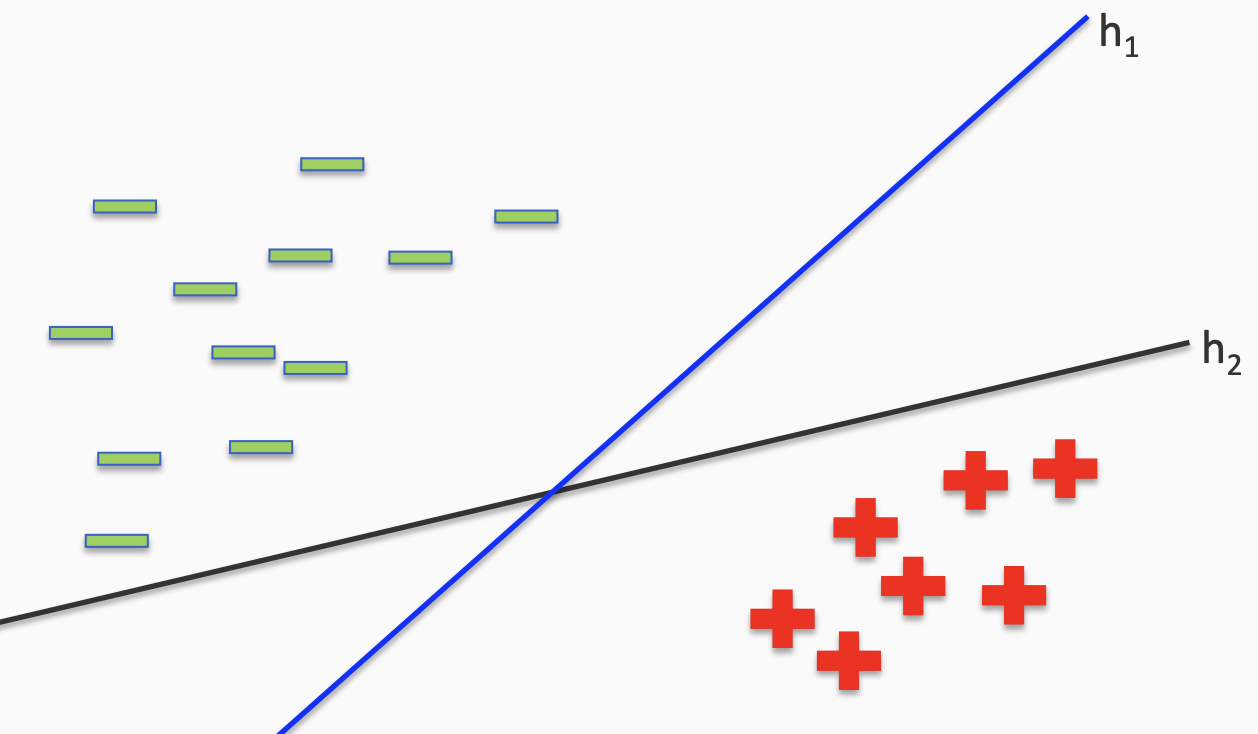
\includegraphics[width=0.5\textwidth]{figures/perceptron_margin}
    \end{figure}
    \fillwithlines{2em}
    \begin{soln}
    Here is a brief algorithm:
    \begin{itemize}
        \item We would first normalize the input samples. Initialize $\mathbf{w}_1=\mathbf{y} \mathbf{x}$, where $\mathbf{x}$ is the first example seen and initialize $t$ to 1.
        \item Predict positive if $\frac{\mathbf{w}_t \cdot \mathbf{x}}{\left\|\mathbf{w}_t\right\|} \geq \gamma / 2$, predict negative if $\frac{\mathbf{w}_t \cdot \mathbf{x}}{\left\|\mathbf{w}_t\right\|} \leq-\gamma / 2$, and consider an example to be a margin mistake when $\frac{\mathbf{w}_t \cdot x}{\left\|\mathbf{w}_t\right\|} \in(-\gamma / 2, \gamma / 2)$.
        \item On a mistake (incorrect prediction or margin mistake), update as in the standard Perceptron algorithm: $\mathbf{w}_{t+1} \leftarrow \mathbf{w}_t+\mathbf{y} \mathbf{x} ; t \leftarrow t+1$.
    \end{itemize}
    \end{soln}   
    \begin{qauthor}
    Varsha, If the students come up with the second and third parts to some extent, we can give them complete credit.
    \end{qauthor}

    \begin{qtester}
   This may be a little difficult. We do not talk about margins much until SVMs. I don't think this was covered with Perceptron. Which learning objective is this addressing?
    \end{qtester}

    \part In this question you will have to answer some questions regarding the perceptron algorithm.
    \begin{subparts}
    \subpart[1] \textbf{Short Answer: }Consider a supervised learning problem with N examples, each of which is a point in d-dimensional space. Let us say our perceptron has converged after t iterations. What is the runtime complexity of the algorithm as a function of N, d, and t? Give a brief explanation of your answer.
    \fillwithlines{1em}
    \begin{soln}
         O(N * d * t), t iterations, each iteration we would perform a dot product which takes O(d) for N samples.
    \end{soln}
    \begin{qauthor}
    Varsha, Implement the perceptron algorithm for binary classification
    \end{qauthor}

    \subpart[2]\textbf{Short Answer: }Let us say we have a learning problem where each input is of d dimensions. Each of these d feature values can only take values 0 or 1. Design a perceptron which classifies the samples as positive if the number of 1s in the feature values of the input is more than the number of 0s. 
    
    \fillwithlines{1em}
    \begin{soln}
         We can have a perceptron where all the weights for d features is 1, and bias term is ceil(-(d+1)/2). (We can get this solution algebraically)
    \end{soln}
    \begin{qauthor}
    Varsha
    \end{qauthor}
    \end{subparts}
\end{parts}

\subsection{Linear Regression}
\begin{parts}

\part[2] \textbf{Numerical answer:} For a linear regression model assume the learning rate $\alpha$ is $0.1$ and the initial value of parameters $\theta_0$ is $0$ and $\theta_1$ is $1$. The training set has 3 samples with the following values:
\begin{center}
    \begin{tabular}{c|c}
		\hline
		x_1& y\\
	    \hline
		1&3 \\
  		3&5 \\
            4&8 \\
		\hline
    \end{tabular}
\end{center}

Use the gradient descent update rule to find the value of parameter $\theta_1$ after one iteration. 
    \begin{tcolorbox}[fit,height=1cm, width=2cm, blank, borderline={1pt}{-2pt}]
    %solution
    \end{tcolorbox}
    \begin{soln}
    1.8
    \end{soln}
    \begin{qauthor}
    Kushagra Agarwal, Implement learning for Linear Regression using ONE optimization technique:(2) gradient descent (the others are saved for Exam 2).
    \end{qauthor}

\part[2] \textbf{Numerical answer:} Suppose you have a quadratic function  $f(x) = 6x^2 - 3x + 5$ that you want to minimize using gradient descent. Apply the gradient descent algorithm with a learning rate $\alpha$ of $0.1$, starting from an initial guess $x=2$ and calculate the new value of $x$ after one iteration.
    \begin{tcolorbox}[fit,height=1cm, width=2cm, blank, borderline={1pt}{-2pt}]
    %solution
    \end{tcolorbox}
    \begin{soln}
    $-0.1$
    \end{soln}
    \begin{qauthor}
    Kushagra Agarwal, Apply gradient descent to optimize a function
    \end{qauthor}
    
\part Suppose that we are an adversary that wants to do \textit{as poorly as possible} on some decision task. This logic has applications to fields such as robust and fair ML, where developers must consider the worst-case performance of their model over a set of plausible distributions of individuals. However, rather than investigating worst-case performance over distributions, we consider worst-case performance on a fixed set $X, Y$, over \textbf{model parameters} $\theta$. 

\begin{subparts}
    
    \subpart[2] \textbf{Short answer}: Write the objective function for this new problem setup, using the variables $\theta \in \mathbb{R}^{M}$ to denote the parameter of interest, $\hat{\theta}$ for the estimated solution of interest, and $J$ to represent the (arbitrary) objective function.

    \begin{soln}
    \begin{align*}
        \hat{\theta} = \argmax_{\theta \in \mathbb{R}^M} J(\theta)
    \end{align*}
    \end{soln}
    
    \subpart[2] \textbf{Short answer}: Explain why the use of this objective for linear regression is flawed in an unconstrained optimization setting.
    
    \begin{soln}
        Note that in this setting, we can make $\hat{\theta}$ \textbf{arbitrarily bad} leading to degenerate solutions if no constraints are imposed on its values. For example, you could adversarially set the values within $\theta$ to approach $\pm \inf$, and as you keep shifting $\theta$ to arbitrarily large-magnitude values, your predictions would become arbitrarily farther away from the solutions, meaning finding an argmax could entail $\theta_i = \pm \inf, 0 \leq i \leq M$.
    \end{soln}

    \subpart[2] \textbf{Short answer}: Propose one way we could ameliorate the above problem.

    \begin{soln}
        Imposing constraints on $\hat{\theta}$, e.g. $||\hat{\theta}||_2^2 \leq \epsilon, \epsilon \in \mathbb{R}$, or $|\hat{\theta} - \theta^*| \leq \epsilon$, where $\theta^*$ denotes the value of $\theta$ that minimizes the objective functions (e.g. OLS solution for 'regular' linear regression; we say that the worst-case $\hat{\theta}$ cannot stray too far from a 'good' solution to the optimization problem)
    \end{soln}
\end{subparts}

\begin{qauthor}
    (1) Kevin, (2) objective functions/closed form solutions in OLS
\end{qauthor}

\part[2] \textbf{Short answer}:
    Consider the following loss function $\ell$, which uses the \textit{absolute value} of the residual between a label $Y$ and its estimation $\hat{Y} = \theta X + \theta_0$, where $X$ is a feature vector and $\theta, \theta_0$ represent a learned set of parameters for regression:
    \begin{align*}
        \ell(Y, \hat{Y}) = |Y - \hat{Y}|
    \end{align*}
    We would like to use $\ell$ in place of residual sum of squares (RSS) when identifying loss over a matrix of training data $X$ and labels $Y$ containing $n$ individuals each, e.g.

    \begin{align*}
        L(X, Y) = \frac{1}{n} \sum_{i = 1}^{n} \ell(Y_i, \theta(X_i) + \theta_0)
    \end{align*}
    
    If possible, provide the closed-form solution to an adaptation of linear regression using the sum of absolute values of residuals $\ell$ in place of RSS. If this is not possible, provide a brief justification as to why, and a potential alternative solution.
    
\begin{soln}
    This is not possible, because the loss function is not differentiable w.r.t. $\hat{y}$ and therefore $x$. As a result, the MLE methods that make a closed-form solution for OLS possible are not applicable to $\ell$. Linear programming/algorithmic approaches on the data should still be able to yield an approximate solution, however.
\end{soln}

\begin{qauthor}
    (1) Kevin, (2) importance of differentiable loss functions in developing closed-form sollutions; consideration of algorithmic techniques for optimization
\end{qauthor}

\part[2] \textbf{Select one}: Consider the following methods of determining whether gradient descent for (unconstrained) OLS linear regression has converged yet. Which of the following would not be valid ways of doing so?

\begin{checkboxes}
    \choice stopping once the L2 norm of the gradient w.r.t. the estimated solution $\theta$ is less than some constant $\epsilon$
    \choice stopping after a fixed set of iterations of gradient descent
    \choice stopping once the L2 norm of the solution $\theta$ is less than a threshold $\epsilon$
    \choice stopping once the change in the objective function from one iteration $t$ to the next iteration $t+1$ is less than a threshold $\epsilon$, e.g. $J(\theta_t; X,Y) - J(\theta_{t+1}; X,Y) \leq \epsilon$
\end{checkboxes}

\begin{soln}
    C
\end{soln}

\begin{qauthor}
    (1) Kevin, (2) stopping conditions in gradient descent for OLS
\end{qauthor}

\begin{qauthor}
    (1) Kevin, (2) importance of differentiable loss functions in developing closed-form sollutions; consideration of algorithmic techniques for optimization
\end{qauthor}
\end{parts}

\subsection{Other/Miscellaneous/Multiple Topics}
\begin{parts}


\part[2] \textbf{Select one:} When we train machine learning models, why do we try to minimize the training error instead of directly minimizing the true error?
    \begin{checkboxes}
     \choice It is possible to calculate the true error, but it is very computationally expensive to find it, so we use the training error instead.
     \choice We don't. With a reasonably large dataset, training error and true error are exactly the same thing.
     \choice Determining the true error requires you to have access to a training dataset that contains every single possible input and output to the model.
     \choice Using the training error instead of the true error guarantees that your learning algorithm will converge.
    \end{checkboxes}
    \begin{soln}
    C. You cannot calculate the true error, since you need to have access to every single point in the domain to do so (and also an accurate error metric). 
    \end{soln}
    \begin{qauthor}
    Rohan Chawla, Explain the difference between true error and training error.
    \end{qauthor}

\end{parts}





% \clearpage
\sectionquestion{CNNs \& RNNs}

\begin{parts}

\part For this question, you will consider the following kernel: 

\begin{center}
    \begin{tabular}{ |c|c|c| } 
     \hline
     -1 & -1 & -1 \\ \hline
     -1 & 1 & 1 \\ \hline
     -1 & 1 & 1 \\ \hline
    \end{tabular}
\end{center}

\begin{subparts}
    \subpart[1] \textbf{Numerical answer:} What is the output of convolving this kernel with the following matrix?

    \begin{center}
        \begin{tabular}{ |c|c|c| } 
         \hline
         4 & 2 & -1 \\ \hline
         0 & 3 & -1 \\ \hline
         1 & -1 & 3 \\ \hline
        \end{tabular}
    \end{center}
    
    \begin{tcolorbox}[fit,height=1cm, width=2cm, blank, borderline={1pt}{-2pt}]
        \begin{soln}
            -2
        \end{soln}
    \end{tcolorbox}
    
    \subpart[1] \textbf{Short answer:} Using \textbf{two or fewer words}, describe what feature the kernel above would detect in an image. \textbf{Hint:} focus on what shapes/patterns in an image would have the greatest magnitude when convolved with this kernel. 
    \fillwithlines{4em}
    \begin{soln}
        Corners
    \end{soln}
\end{subparts}
\begin{qauthor}
    Henry
\end{qauthor}

\part Suppose you are learning a CNN where the first convolutional layer takes color images as inputs, represented as 3 10$\times$10 channels. This layer uses 5$\times$5 kernels \emph{with no bias term} and outputs a single channel. It also uses a padding of 2 and a stride of 3. 

\begin{subparts}
    \subpart[1] \textbf{Numerical answer:} How many learnable parameters does this convolutional layer have?
    \begin{tcolorbox}[fit,height=1cm, width=2cm, blank, borderline={1pt}{-2pt}]
        \begin{soln}
            $3*5*5 = 75$
        \end{soln}
    \end{tcolorbox}
    
    \subpart[1] \textbf{Numerical answer:} What is the dimensionality of the output channel?
    \begin{tcolorbox}[fit,height=1cm, width=2cm, blank, borderline={1pt}{-2pt}]
        \begin{soln}
            4$\times$4
        \end{soln}
    \end{tcolorbox}
\end{subparts}
\begin{qauthor}
    Henry
\end{qauthor}

\clearpage
\part[2] \textbf{Select all that apply:} Neural the Narwhal is trying to train a CNN with one convolutional layer followed by a fully-connected layer. Unfortunately he can't get backpropagation to run on his state-of-the-art Commodore Amiga because his model has too many parameters. Which of the following changes to his architecture \emph{could} decrease the total number of learnable parameters in Neural's CNN?
{%
    \checkboxchar{$\Box$} \checkedchar{$\blacksquare$} % change checkbox style locally
    \begin{checkboxes}
     \choice Increase the size of his kernels
     \choice Increase the stride in his convolutional layer
     \choice Add a max pooling layer between the convolutional and fully-connected layers
     \choice Add an additional convolutional layer before the fully-connected layer
     \choice None of the above
    \end{checkboxes}
}
\begin{soln}
    A, B, C and D
\end{soln}
\begin{qauthor}
    Henry 
\end{qauthor}

\part[2] \textbf{Matching:} Markov the Narwhal is trying to train a machine learning model to predict the current outdoor temperature. He has lots of different kinds of data that he could potentially train his model with. For each kind of training data listed below, select the deep learning architecture that is \emph{best} suited to work with it; each option may be used multiple times or not at all.  
\\
\begin{mdframed}[innerrightmargin=20pt]
    \begin{multicols}{2}
        \begin{enumerate}[label=(\alph*)]
            \item Fully-connected feed-forward neural network
            \item Convolutional neural network
            \item Recurrent neural network
            \item Bidirectional recurrent neural network
        \end{enumerate}
    \end{multicols}
\end{mdframed}
\begin{center}
    \begin{tabular}{r l}
        A picture of the sky outside Markov's window & \begin{tcolorbox}[fit,height=1cm, width=2cm, blank, borderline={1pt}{-2pt}]
            %solution
        \end{tcolorbox} \\
        The previous hourly temperatures for the past 10 hours & \begin{tcolorbox}[fit,height=1cm, width=2cm, blank, borderline={1pt}{-2pt}]
            %solution
        \end{tcolorbox} \\
        The current outdoor temperature at 10 nearby cities & \begin{tcolorbox}[fit,height=1cm, width=2cm, blank, borderline={1pt}{-2pt}]
            %solution
        \end{tcolorbox} \\
        A transcript of the local news's morning weather report & \begin{tcolorbox}[fit,height=1cm, width=2cm, blank, borderline={1pt}{-2pt}]
            %solution
        \end{tcolorbox}
    \end{tabular}
\end{center}
    
\begin{soln}
    (b), (c), (a), (d) (or (c)...)
\end{soln}
\begin{qauthor}
    Henry
\end{qauthor}
    
\part Let $L$ be the length of the input sequence to some RNN model.
\begin{subparts}
    \subpart[1] \textbf{Select one:} How does the number of learnable parameters in the RNN scale as $L$ increases?
    \begin{checkboxes}
        \choice $O(1)$: the number of learnable parameters does not depend on $L$
        \choice $O(\log L)$: the number of learnable parameters grows logarithmically as $L$ increases
        \choice $O(L)$: the number of learnable parameters grows linearly as $L$ increases
        \choice $O(L^2)$: the number of learnable parameters grows quadratically as $L$ increases
    \end{checkboxes}
    \begin{soln}
        A
    \end{soln}

    \subpart[1] \textbf{Select one:} How does the computational cost of a single forward pass through the RNN model scale as $L$ increases?
    \begin{checkboxes}
        \choice $O(1)$: the computational cost does not depend on $L$
        \choice $O(\log L)$: the computational cost grows logarithmically as $L$ increases
        \choice $O(L)$: the computational cost grows linearly as $L$ increases
        \choice $O(L^2)$: the computational cost grows quadratically as $L$ increases
    \end{checkboxes}
    \begin{soln}
        C
    \end{soln}
\end{subparts}
\begin{qauthor}
    Henry
\end{qauthor}

\part Recall that a bidirectional RNN is defined by the following set of equations, which also correspond to the figure on the left: 
\begin{align*}
    \vcenter{\hbox{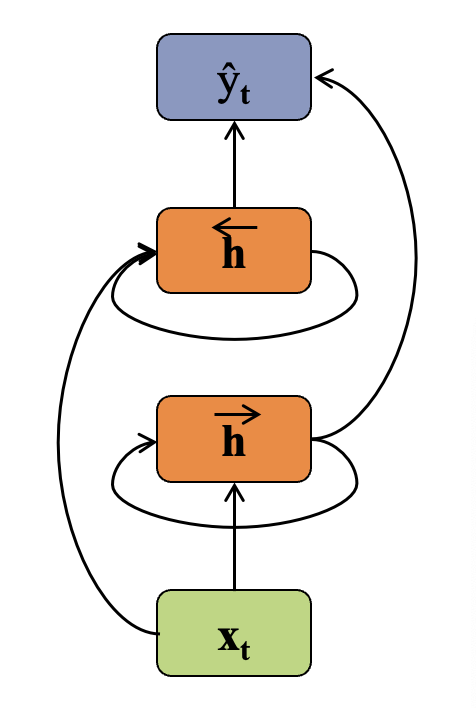
\includegraphics[width=5cm]{exam3/figures/brnn.png}}}
    \qquad
    \begin{aligned}
        \overrightarrow{\hv}_t &= \mathcal{H}(W_{x\overrightarrow{\hv}}\xv_t+W_{\overrightarrow{\hv}\overrightarrow{\hv}}\overrightarrow{\hv}_{t-1}+b_{\overrightarrow{\hv}}) \\ 
        \overleftarrow{\hv}_t &= \mathcal{H}(W_{x\overleftarrow{\hv}}\xv_t+W_{\overleftarrow{\hv}\overleftarrow{\hv}}\overleftarrow{\hv}_{t+1}+b_{\overleftarrow{\hv}}) \\ 
        \hat{y}_t &= W_{\overrightarrow{\hv}y}\overrightarrow{\hv}_t+W_{\overleftarrow{\hv}y}\overleftarrow{\hv}_t+b_y
    \end{aligned}
\end{align*}

\begin{subparts}
    \subpart[3] \textbf{Select all that apply:} Given sequences of length 3 of the form \\ $(\xv_1, y_1, \xv_2, y_2, \xv_3, y_3)$ which of the following quantities does $\overleftarrow{\hv}_2$ depend on?
    {%
    \checkboxchar{$\Box$} \checkedchar{$\blacksquare$} % change checkbox style locally
    \begin{checkboxes}
     \choice $\overrightarrow{\hv}_2$
     \choice $\xv_3$
     \choice $y_3$
     \choice $\hat{y}_3$
     \choice $\xv_1$
     \choice $W_{\overleftarrow{\hv}\overleftarrow{\hv}}$
     \choice None of the above
    \end{checkboxes}
    }
    \begin{soln}
        B, F
    \end{soln}

    \clearpage
    
    \subpart[3] \textbf{Select all that apply:} If the loss function is defined as \\ $\mathcal{L}=\sum_{t=1}^3 (y_t-\hat{y}_t)^2$, which of the following quantities does $\nicefrac{\partial \mathcal{L}}{\partial \overleftarrow{\hv}_2}$ depend on?
    {%
    \checkboxchar{$\Box$} \checkedchar{$\blacksquare$} % change checkbox style locally
    \begin{checkboxes}
     \choice $\nicefrac{\partial \mathcal{L}}{\partial \overleftarrow{\hv}_1}$
     \choice $\hat{y}_3$
     \choice $y_3$
     \choice $y_2$
     \choice $\nicefrac{\partial \mathcal{L}}{\partial W_{x\overrightarrow{\hv}}}$
     \choice $W_{\overleftarrow{\hv}y}$
     \choice None of the above
    \end{checkboxes}
    }
    \begin{soln}
        A, D, F
    \end{soln}
\end{subparts}
\begin{qauthor}
    Henry
\end{qauthor}
\end{parts}
\clearpage
% \sectionquestion{Recurrent Neural Networks (RNNs)}

\begin{parts}
\part[0] TODO
\end{parts}
% \clearpage
\sectionquestion{Module-Based AutoDiff \& Attention}

\begin{parts}

\part[2] \textbf{Fill in the blank:} Complete the following paragraph about module-based automatic differentiation by circling the best of the provided options for each of blanks: 

\doublespacing
\begin{quote}
        In module-based automatic differentiation, each module is added to the tape during the \underline{\quad forward \quad / \quad backward \quad /} pass. The tape is represented by a \underline{\quad stack \quad / \quad queue \quad /} and module-based automatic differentiation removes modules from the tape in \underline{\quad topological \quad / \quad reverse topological \quad /} order with respect to the network's implied computation graph. 
\end{quote}
\singlespacing

\begin{soln}
    In module-based automatic differentiation, each module is added to the tape during the forward pass. The tape is represented by a stack and module-based automatic differentiation removes modules from the tape in reverse topological order with respect to the network's implied computation graph. 
\end{soln}
\begin{qauthor}
    Henry
\end{qauthor}

\part[2] \textbf{Select all that apply:} Which of the following statements is/are valid reasons to prefer module-based automatic differentiation over the procedural approach?
{%
    \checkboxchar{$\Box$} \checkedchar{$\blacksquare$} % change checkbox style locally
    \begin{checkboxes}
         \choice Module-based automatic differentiation tends to return a better set of weights at convergence (in terms of minimizing the neural network loss function) when run for the same number of epochs of SGD
         \choice Module-based automatic differentiation allows for more efficient experimentation with deep learning architectures that stack many multi-layer units together (in terms of minimizing the lines of code)
         \choice Module-based automatic differentiation eliminates the need to write backwards methods for certain modules if they are built using only modules with backwards methods
         \choice Module-based automatic differentiation allows for the use of certain deep learning architectures that cannot be trained using the procedural approach
         \choice None of the above
    \end{checkboxes}
}
\begin{soln}
    B and C
\end{soln}
\begin{qauthor}
    Henry
\end{qauthor}

\part[1] \textbf{Math:} Suppose you have a single attention head that takes as input sequences of length $L$ where each token in the sequence is $D$-dimensional. It computes scaled dot-product attention using $C$-dimensional query vectors and outputs an $M$-dimensional embeddings for each token. How many parameters does this attention head have? 
\begin{tcolorbox}[fit,height=1cm, width=2cm, blank, borderline={1pt}{-2pt}]
    \begin{soln}
        $2DC+DM$
    \end{soln}
\end{tcolorbox}
\begin{qauthor}
    Henry
\end{qauthor}

\clearpage

\part[2] \textbf{Select all that apply:} Which of the following statements about multi-head attention is/are correct?
    {%
    \checkboxchar{$\Box$} \checkedchar{$\blacksquare$} % change checkbox style locally
    \begin{checkboxes}
         \choice Each head learns its own set of value weights $W_v$
         \choice A single set of query weights $W_q$ is learned and shared across all heads
         \choice The dimensionalities of the query vectors must be the same across all heads
         \choice The outputs of each head are added together to form the final embedding
         \choice None of the above
    \end{checkboxes}
    }
    \begin{soln}
        A
    \end{soln}
    \begin{qauthor}
        Kushagra Agarwal, Describe the role of keys, queries and values in an attention module.
    
        Lightly edited by Henry
    \end{qauthor}

\part[2] \textbf{Short answer:} In 2-3 concise sentences, define position embeddings in the context of a transformer language model and explain why they are important to include in a transformer language model.
\fillwithlines{12em}
\begin{soln}
    Position embeddings are vectors $p_t$ that capture information about where in the sequence each token is. Transformers require position embeddings because otherwise they have no ability to infer the relative or absolute position of tokens in their inputs i.e., two sequences with all the same tokens but in a different order would appear identical to a transformer language model. 
\end{soln}
\end{parts}
\clearpage
\sectionquestion{MDPs and Value/Policy Iteration}

\begin{parts}


\part Suppose we wish to learn to play the classic side-scrolling computer game Lemmings. For the first level, each state $s=(s_{ij}, s_d)$ in state space $\Sc$ contains the lemming's position ($s_{ij}$), the lemming's direction ($s_d \in \{\text{left}, \text{right}\}$). The action space is $\Ac = \{$ \texttt{continue}, \texttt{dig} $\}$. 
\begin{itemize}
    \item The \texttt{continue} action allows the lemming to walk one tile in its current direction (left or right). 
    \\
    \textit{Example:} From  $s=(s_{22}, \text{right})$ taking \texttt{continue} yields $s=(s_{23}, \text{right})$.
    
    \item Physics applies: if the direction $s_d$ leads into solid tile (brown or gray), the lemming position remains unchanged but its direction switches. 
    \\
    \textit{Example:} From $s=(s_{47}, \text{right})$ taking \texttt{continue} yields $s=(s_{47}, \text{left})$.
    
    \item Gravity applies: If the lemming is above a non-solid tile (white or blue), it will fall down one tile regardless of its direction. %\textit{Example:} if the lemming is moving right from $s_{55}$, in one turn it moves to $s_{56}$, and in two turns to $s_{46}$. 
    \\
    \textit{Example:} From $s=(s_{55}, \text{right})$ taking \texttt{continue} yields $s=(s_{56}, \text{right})$.
    \\
    \textit{Example:} From $s=(s_{56}, \text{right})$ taking any action yields $s=(s_{46}, \text{right})$.
    
    \item The \texttt{dig} action allows the lemming to move down through a dirt tile (brown). 
    Taking the \texttt{dig} action over a non-dirt tile leads to the same result as if the \texttt{continue} action were taken.
    \\
    \textit{Example:} From $s=(s_{53}, \text{left})$ taking \texttt{dig} yields $s=(s_{43}, \text{left})$.
    \\
    \textit{Example:} From $s=(s_{43}, \text{left})$ taking any action yields $s=(s_{33}, \text{left})$.
\end{itemize}
The goal tile (yellow) and the water tiles (blue) are terminal states. The reward function returns $+100$ for entering the goal tile and $-100$ for entering a water tile. Assume $\gamma = 0.9$.

    \begin{center}
        \begin{tikzpicture}
        
            % Coloring specific cells
            \foreach \i in {1,...,9} {
                \fill[gray] (\i-1,5) rectangle (\i,6); % top row
                \fill[gray] (\i-1,0) rectangle (\i,1); % bottom row  
            }
            \foreach \j in {1,...,6} {
                \fill[gray] (0,\j-1) rectangle (1,\j); % left col
                \fill[gray] (8,\j-1) rectangle (9,\j); % right col  
            }
            \foreach \i in {3,...,5} {
                \fill[brown] (\i-1,3) rectangle (\i,4); 
            }
            \foreach \i in {6,...,7} {
                \fill[brown] (\i-1,2) rectangle (\i,3); 
            }
            \fill[brown] (1,3) rectangle (2,4);
            \fill[brown] (2,3) rectangle (3,4);
            
            \fill[blue] (4,0) rectangle (5,1);
            \fill[blue] (3,0) rectangle (4,1);  
            \fill[yellow] (7,1) rectangle (8,2);
            
            \fill[gray] (7,3) rectangle (8,4);
            \fill[gray] (8,3) rectangle (9,4);

            \node at (1.5,4.5) {
\includegraphics[width=0.8cm]{figures/lemming.png}};
            
            \draw[step=1cm] (0,0) grid (9, 6);
            
            % Loop to place s_{ij} in each cell
            \foreach \i in {1,...,9} {
                \foreach \j in {1,...,6} {
                    % Places s_{ij} at the center of the cell (\i+1,\j+1)
                    \node at (\i+0.75-1,\j+0.75-1) {$s_{\j\i}$};
                }
            }
            
        \end{tikzpicture}
    \end{center}

\begin{subparts}

\subpart[1] \textbf{Numerical answer:} What is $V^*(s)$ for $s=(s_{27}, \text{right})$?
    \begin{tcolorbox}[fit,height=1cm, width=2cm, blank, borderline={1pt}{-2pt}]
    %solution
    \end{tcolorbox}
    \begin{soln}
    $+100$
    \end{soln}
    \begin{qauthor} Matt    \end{qauthor}

\clearpage
    
\subpart[1] \textbf{Numerical answer:} What is $V^*(s)$ for $s=(s_{27}, \text{left})$?
    \begin{tcolorbox}[fit,height=1cm, width=2cm, blank, borderline={1pt}{-2pt}]
    %solution
    \end{tcolorbox}
    \begin{soln}
    $0.9^2 * -100$
    \end{soln}
    \begin{qauthor} Matt    \end{qauthor}
    
\subpart[2] \textbf{Select one:} Suppose we are in a state $s=(s_{ij}, s_d)$ where $s_{ij} = s_{46}$. Is the action $a=$dig always an optimal action? \textbf{Briefly justify your answer.}
    \begin{checkboxes}
     \choice Yes
     \choice No
    \end{checkboxes}    
    \fillwithlines{8em}
    \begin{soln}
    No. If $s_d=$right, it is optimal. If $s_d=$left, it would cause the lemming to walk into the water, so $a=$continue should be chosen instead.
    \end{soln}
    \begin{qauthor} Matt    \end{qauthor}

\subpart[1] \textbf{Select one:} How many optimal policies are there for this problem?
    \begin{checkboxes}
     \choice zero
     \choice one
     \choice an integer greater than one
     \choice infinitely many
    \end{checkboxes}
    \begin{soln}
    an integer greater than one
    \end{soln}
    \begin{qauthor} Matt    \end{qauthor}

\subpart[1] \textbf{Numerical answer:} What is $Q^*(s,a)$ for $s=(s_{54}, \text{right})$ and $a=\texttt{dig}$?
    \begin{tcolorbox}[fit,height=1cm, width=2cm, blank, borderline={1pt}{-2pt}]
    %solution
    \end{tcolorbox}
    \begin{soln}
    $0.9^3 * -100 = -72.9$
    \end{soln}
    \begin{qauthor} Matt    \end{qauthor}

\subpart[1] \textbf{Select one:} Does this environment have stochastic transitions or deterministic transitions?
    \begin{checkboxes}
     \choice stochastic transitions
     \choice deterministic transitions
    \end{checkboxes}
    \begin{soln}
    deterministic transitions
    \end{soln}
    \begin{qauthor} Matt    \end{qauthor}
    
    
\end{subparts}


\part[2] \textbf{Select all that apply:} Which of the following is true of a Markov decision process (MDP)?
    {%
    \checkboxchar{$\Box$} \checkedchar{$\blacksquare$} % change checkbox style locally
    \begin{checkboxes}
     \choice An MDP defines one way that the state, action, reward tuples are gathered for reinforcement learning.
     \choice The components of an MDP include a state space, action space, transition probabilities, reward function, and policy.
     \choice Every state/action space of finite size consists of exactly one optimal policy.
     \choice The Bellman equations are a recursive definition of the optimal policy.
     \choice None of the above
    \end{checkboxes}
    }
    \begin{soln}
    A, B
    \end{soln}
    \begin{qauthor}
    Matt
    \end{qauthor}

\part[1] \textbf{True or False:} Value iteration learns the optimal value function from which we can infer the optimal policy. By contrast, policy iteration learns the optimal policy from which we \emph{cannot} infer the optimal value function.
    \begin{checkboxes}
     \choice True 
     \choice False
    \end{checkboxes}
    \begin{soln}
    False, we can infer the optimal value function from the optimal policy.
    \end{soln}
    \begin{qauthor}
    Matt
    \end{qauthor}


\end{parts}
\clearpage
\sectionquestion{Q-Learning and Deep RL}

\begin{parts}

\part Bocchi and Dora are both running tabular Q-learning on the same environment with unknown nondeterministic transitions. 
The two use the exact same parameters, except the value for $\epsilon$ in their $\epsilon$-greedy action selection (i.e. choose a random action with probability $\epsilon$, and a greedy action with probability $(1-\epsilon)$).
Since Bocchi does not like exploring, she sets $\epsilon = 0$. Meanwhile, Dora loves exploring so she sets $\epsilon = 1$.
%
Assume the discount factor $\gamma$ satisfies $0 \leq \gamma < 1$, rewards are finite and bounded, Q-values are initialized to zero, and learning rate $\alpha_t$ follows the schedule $\alpha_t = \frac{1}{t+1}$.

    \begin{subparts}
        \subpart[2] \textbf{Select one:} Over an arbitrarily large number of steps, is Bocchi's Q-learning algorithm guaranteed to converge to the optimal Q-value function? \textbf{Explain in one sentence.}
        \begin{checkboxes}
            \choice Yes
            \choice No
        \end{checkboxes}
        \fillwithlines{5em}
        \begin{soln}
        No, since Bocchi's algorithm isn't guaranteed to visit every state 
        \end{soln}

        \subpart[2] \textbf{Select one:} Over an arbitrarily large number of steps, is Dora's Q-learning algorthim guaranteed to converge to the optimal Q-value function?  \textbf{Explain in one sentence.}
        \begin{checkboxes}
            \choice Yes
            \choice No
        \end{checkboxes}
        \fillwithlines{5em}
        \begin{soln}
            Yes, since Dora's algorithm is guaranteed to visit every state arbitrarily many times
        \end{soln}

        \begin{comment}
        \subpart[2] \textbf{Short answer:} Why might it be preferable to set $\epsilon$ to a small non-zero constant instead of exactly $0$ or $1$?
        \fillwithlines{7em}
        \begin{soln}
            $\epsilon$-greedy strikes a balance between exploration and exploitation; it is guaranteed to converge unlike a pure greedy strategy and likely to converge faster than a pure random strategy.
        \end{soln}
        \end{comment}
        
    \end{subparts}
        

\begin{qauthor}
    Alex, Identify the conditions under which the Q-learning algorithm will converge to the true value function
\end{qauthor}

\clearpage

\part Consider a supervised online learning problem in which your goal is to minimize the number of mistakes made on a stream of examples $(\xv^{(1)}, y^{(1))}), (\xv^{(2)}, y^{(2))}), \ldots$ where $\xv^{(i)} \in \Rb^M$ and $y^{(i)} \in \{+1, -1\}$ and $y^{(i)} = c^*(\xv^{(i)})$. Assume for all $i \neq j$, $\xv^{(i)} \neq \xv^{(j)}$ and that the model is not able to view any past points after a new one arrives.

In this problem, you will recast this \textit{online learning} problem as a \textit{reinforcement learning} problem by defining your state space $\Sc$, action space $\Ac$, reward function $R(s,a)$, and transition function $\delta(s,a)$. Your goal is to learn a linear model $\hat{y}^{(i)} = h_{\thetav}(\xv^{(i)}) = \text{sign}(\thetav^T\xv^{(i)})$. 

\textbf{(For full credit, all your answers must be in terms of mathematical quantities appearing in the above paragraphs.)}

\begin{subparts}

\subpart[1] \textbf{Short answer:} What is the state at timestep $t$, i.e. $s_{t}$?
    \begin{tcolorbox}[fit,height=1cm, width=4cm, blank, borderline={1pt}{-2pt}]
    %solution
    \end{tcolorbox}
    \begin{soln}
    $\xv^{(t)}$, i.e. the $t$th feature vector
    \end{soln}
    \begin{qauthor}   Matt    \end{qauthor}

\subpart[1] \textbf{Short answer:} Define the state space, $\Sc$.
    \begin{tcolorbox}[fit,height=1.5cm, width=6cm, blank, borderline={1pt}{-2pt}]
    %solution
    \end{tcolorbox}
    \begin{soln}
    $\Rb^M$, i.e. real-valued vectors of length $M$
    \end{soln}
    \begin{qauthor}   Matt    \end{qauthor}

% \subpart[1] \textbf{Short answer:} What is the greedy action at timestep $t$, i.e. $a_{t}$?
%     \begin{tcolorbox}[fit,height=1cm, width=4cm, blank, borderline={1pt}{-2pt}]
%     %solution
%     \end{tcolorbox}
%     \begin{soln}
%     $\hat{y}^{(t)}$, i.e. the $t$th prediction
%     \end{soln}
%     \begin{qauthor}   Matt    \end{qauthor}
    
\subpart[1] \textbf{Short answer:} Define the action space, $\Ac$.
    \begin{tcolorbox}[fit,height=1.5cm, width=6cm, blank, borderline={1pt}{-2pt}]
    %solution
    \end{tcolorbox}
    \begin{soln}
    $\{+1, -1\}$, i.e. assigning a label of $+1$ or $-1$ to $y^{(i)}$
    \end{soln}
    \begin{qauthor}   Matt    \end{qauthor}
    
\subpart[1] \textbf{Short answer:} Define the reward function, $R(s, a) : \Sc \times \Ac \rightarrow \Rb$.
    \begin{tcolorbox}[fit,height=1.9cm, width=8cm, blank, borderline={1pt}{-2pt}]
    %solution
    \end{tcolorbox}
    \begin{soln}
    \begin{align*}
        R(\xv^{(t)}, a) = \begin{cases}
        1 & \text{if } y^{(t)} = a \\
        0 & \text{if } y^{(t)} \neq a 
        \end{cases}
    \end{align*}
    \end{soln}
    \begin{qauthor}   Matt    \end{qauthor}
    
\subpart[1] \textbf{Short answer:} Define the transition function, i.e. $s_{t+1} = \delta(s_t, a_t)$.
    \begin{tcolorbox}[fit,height=1.9cm, width=8cm, blank, borderline={1pt}{-2pt}]
    %solution
    \end{tcolorbox}
    \begin{soln}
    $\delta(\xv^{(t)}, \hat{y}^{(t)}) = \xv^{(t+1)}$
    \end{soln}
    \begin{qauthor}   Matt    \end{qauthor}

% \subpart[1] \textbf{Short answer:} Define the policy, $\pi(s_t) : \Sc \rightarrow \Ac$.
%     \begin{tcolorbox}[fit,height=2cm, width=8cm, blank, borderline={1pt}{-2pt}]
%     %solution
%     \end{tcolorbox}
%     \begin{soln}
%     $\pi(\xv^{(t)}) = h_{\thetav}(\xv^{(t)}) = \text{sign}(\thetav^T \xv^{(t)})$
%     \end{soln}
%     \begin{qauthor}   Matt    \end{qauthor}


\subpart[1] \textbf{Select one:} Which of the following would be the best choice to learn a policy $\pi : \Sc \rightarrow \Ac$?
    \begin{checkboxes}
     \choice value iteration
     \choice policy iteration
     \choice tabular Q-learning
     \choice deep Q-learning
    \end{checkboxes}
    \begin{soln}
    deep Q-learning
    \end{soln}
    \begin{qauthor}   Matt    \end{qauthor}

    
\end{subparts}


\end{parts}
\clearpage
\input{qs-PCA.tex}
\clearpage
\sectionquestion{$K$-Means}

\begin{parts}

\part Suppose we wish to apply $K$-Means to the unlabeled 2D dataset $\Dc = \{ \xv^{(i)} \}_{i=1}^N$ below.

\begin{center}
\begin{tikzpicture}[thick,scale=0.9, every node/.style={transform shape}]
    \begin{axis}[
        axis equal image,
        xmin=-5, xmax=5, xtick={-5,...,5},
        ymin=-3, ymax=3, ytick={-3,...,3},
        xlabel={$x_1$}, ylabel={$x_2$},
        samples=50, grid=major, minor tick num=1,
        xticklabel style={xshift=-0.1cm}]
      \addplot [
            scatter,
            only marks,
            point meta=explicit symbolic,
            scatter/classes={
                a={mark=square*,black}
            },
            nodes near coords*={$\xv^{(\pgfmathprintnumber[frac]\myvalue)}$},
            visualization depends on={\thisrow{myvalue} \as \myvalue},
        ] table [meta=label] {
            x y label myvalue
            -4 -2 a 1
            -2 -2 a 2
            -4 0 a 3
            0 0 a 4
            1 2 a 5
            3 0 a 6
            4 -1 a 7
        };
    \end{axis}
\end{tikzpicture}
\end{center}
 
We set $K=3$ and initialize the cluster centers to $\xv^{(4)}, \xv^{(5)}, \xv^{(7)}$. 
(Assume a single iteration first computes cluster assignments and then computes cluster centers.) 

\begin{subparts}

    \subpart[2] \textbf{Short answer:} What will the partitioning of the points be after the \textbf{first} iteration of $K$-Means? 

        cluster 1: \hspace{3.2cm} cluster 2:  \hspace{3.2cm} cluster 3: 
                
        \begin{tcolorbox}[fit,height=1cm, width=4.5cm, blank, borderline={1pt}{-2pt},nobeforeafter]
        %solution
        \end{tcolorbox}
        \hspace{1em}
        \begin{tcolorbox}[fit,height=1cm, width=4.5cm, blank, borderline={1pt}{-2pt},nobeforeafter]
        %solution
        \end{tcolorbox}
        \hspace{1em}        
        \begin{tcolorbox}[fit,height=1cm, width=4.5cm, blank, borderline={1pt}{-2pt},nobeforeafter]
        %solution
        \end{tcolorbox}
        
        \begin{soln}
        The rubric here should almost certainly NOT be a simple binary check of whether each cluster is correct. That is, there will probably be only a small number of wrong answers and we should group those into equivalence classes.
        
        cluster 1: $\xv^{(1)}, \xv^{(2)}, \xv^{(3)}, \xv^({4})$\\
        cluster 2: $\xv^{(5)}$\\
        cluster 3: $\xv^{(6)}, \xv^{(7)}$\\
        \end{soln}
        \begin{qauthor}
        Matt
        \end{qauthor}

    \subpart[2] \textbf{Short answer:} What will the partitioning of the points be after the \textbf{second} iteration of $K$-Means?

        cluster 1: \hspace{3.2cm} cluster 2:  \hspace{3.2cm} cluster 3: 
                
        \begin{tcolorbox}[fit,height=1cm, width=4.5cm, blank, borderline={1pt}{-2pt},nobeforeafter]
        %solution
        \end{tcolorbox}
        \hspace{1em}
        \begin{tcolorbox}[fit,height=1cm, width=4.5cm, blank, borderline={1pt}{-2pt},nobeforeafter]
        %solution
        \end{tcolorbox}
        \hspace{1em}        
        \begin{tcolorbox}[fit,height=1cm, width=4.5cm, blank, borderline={1pt}{-2pt},nobeforeafter]
        %solution
        \end{tcolorbox}
        
        \begin{soln}
        The rubric here should almost certainly NOT be a simple binary check of whether each cluster is correct. That is, there will probably be only a small number of wrong answers and we should group those into equivalence classes.

        cluster 1: $\xv^{(1)}, \xv^{(2)}, \xv^{(3)}$\\
        cluster 2: $\xv^({4}), \xv^{(5)}$\\
        cluster 3: $\xv^{(6)}, \xv^{(7)}$\\
        \end{soln}
        \begin{qauthor}
        Matt
        \end{qauthor}

    \subpart[1] \textbf{Short answer:} How many total iterations will complete before $K$-Means has converged? (We say that $K$-Means has converged if the next iteration, the cluster assignment will not change.)
        \begin{tcolorbox}[fit,height=1cm, width=4cm, blank, borderline={1pt}{-2pt}]
        %solution
        \end{tcolorbox}        
        \begin{soln}
        2
        \end{soln}
        \begin{qauthor}
        Matt
        \end{qauthor}

\end{subparts}

\part[1] \textbf{True or False:} Given a fixed set of initial cluster centers, $K$-Means \emph{always} converges to the same final cluster assignment, assuming ties in distance are always broken the same way.

    \begin{checkboxes}
     \choice True 
     \choice False
    \end{checkboxes}
    \begin{soln}
    True
    \end{soln}
    \begin{qauthor}
    Matt -- Note for future semesters: We should have labeled the points A, B, C, D,... for easier reading when grading. Also if we had one box for each point and we asked students to simply label them with cluster IDs, then we could auto-grade with Hamming loss.
    \end{qauthor}

\begin{comment}
\part[1] \textbf{True or False:} $K$-Means++ initialization strategy never selects an outlier point as initial cluster centers.

    \begin{checkboxes}
     \choice True 
     \choice False
    \end{checkboxes}
    \begin{soln}
    False
    \end{soln}
    \begin{qauthor}
    Matt
    \end{qauthor}
\end{comment}

\end{parts}
\clearpage
\sectionquestion{Ensemble Methods}

\begin{parts}

\part Graddyant is training a random forest for binary classification on samples $\{(\xv^{(i)}, y^{(i)}\}_{i=1}^n$.
In order to reduce variance, Graddyant applies an extreme form of sample bagging, training each decision tree with only one sample. Assume decision trees are trained using the standard greedy algorithm ID3 used previously in this class, with information gain as the splitting criterion, with no pruning.
\begin{subparts}
\subpart[1] \textbf{Numerical answer:} What is the depth of the largest decision tree in the random forest?
    \begin{tcolorbox}[fit,height=1cm, width=2cm, blank, borderline={1pt}{-2pt}]
    %solution
    \end{tcolorbox}
    \begin{soln}
    0, the root node is already pure and majority vote is sufficient
    \end{soln}


\subpart[2] \textbf{Short answer:} As the number of trees increases, what classifier does Graddyant's random forest resemble in expectation? Why?
    \fillwithlines{10em}
    \begin{soln}
    Majority vote. We get an approximately equal number of trees per sample, and each tree always votes for the label of that sample, so the unweighted majority vote over the forest approximates a majority vote over the data.
    \end{soln}

\subpart[2] \textbf{Select all that apply:} Select all of the following that apply to Graddyant's random forest.
    {%
    \checkboxchar{$\Box$} \checkedchar{$\blacksquare$} % change checkbox style locally
    \begin{checkboxes}
     \choice Each decision tree has low variance.
     \choice Each decision tree has high variance.
     \choice The ensemble has low variance.
     \choice The ensemble has high variance.
     \choice None of the above
    \end{checkboxes}
    }
    \begin{soln}
    A, C. Both the decision tree and ensemble resemble majority vote, high bias low variance.
    \end{soln}
\end{subparts}
    \begin{qauthor}
    Abhi. Ensemble Methods: Bagging

Implement random forests.

Discuss the relation in bagging between the sample size and variance of the base classifier/regressor.

    \end{qauthor}

\clearpage

\part[2] \textbf{Short answer:} At his new company Tweetstatok, Melon Husk asks his employees to speed up their implementation of AdaBoost. He instructs them to ditch the sequential training of weak learners and to instead \emph{train each weak learner in parallel independently and then learn all the weights for the ensemble at once}. The employees chuckle quietly at Melon Husk's naivety. Explain why this approach is not likely to produce the same results as the standard AdaBoost.
% OLD VERSION: Melon Husk is trying to speed up his implementation of AdaBoost at his new company Tweetstatok. Melon decides to try training each weak learner in parallel instead of training weak learners serially, then learn all the weights for the ensemble at once. Will this produce the same results as standard AdaBoost? Why or why not?
    \fillwithlines{10em}
    \begin{soln}
    It won't work, can't update weight distribution based on error of one weak learner to train the next if they're learned in parallel.
    \end{soln}
    \begin{qauthor}
    Abhi. Ensemble Methods: Boosting

    Implement AdaBoost
    \end{qauthor}

\end{parts}
\clearpage
\sectionquestion{Recommender Systems}

\begin{parts}

\part Neural the Narwhal asks his friends (6 users) to rate their favorite sea animals (8 items). He has a sparse ratings matrix of size $6 \times 8$, and he wants to use collaborative filtering to factor this matrix into a user matrix and an item matrix.

\begin{subparts}

    \subpart[2] \textbf{Select All That Apply:}  He thinks, since each latent feature captures information about the underlying data, he wants to factor the user matrix $\Uv$ into size $6 \times 10000$ and the item matrix $\Vv$ into size $8 \times 10000$. Is Neural's choice of $10000$ latent features a reasonable decision?
    {%
    \checkboxchar{$\Box$} \checkedchar{$\blacksquare$} % change checkbox style locally
    \begin{checkboxes}
     \choice Yes, because more latent features are able to capture more data about the factors that go into the ratings, thus leading to model that generalizes better.
     \choice Yes, because after these matrices are learned, predictions will be made on new users, causing the user matrix to grow.
     \choice No, because the matrices that are learned may overfit on the dataset.
     \choice No, because the matrix cannot be factored at all unless the number of latent features is $\min(6,8)$.
     \choice None of the above
    \end{checkboxes}
    }
    \begin{soln}
    C
    \end{soln}
    \begin{qauthor}
    Emily (edited by Matt), Recommender Systems\\
    AFTER FEEDBACK: took by taking out line saying that Neural is wrong and reword question to not imply if this is a good or bad method. changed short answer into select all that apply options.
    \end{qauthor}

    \uplevel{Neural now tries using only 2 features in the latent space, so the user matrix $\Uv$ is of size $6 \times 2$ and so the item matrix $\Vv$ is of size $8 \times 2$.
    Suppose an oracle provides a new user vector $\uv_i \in \Rb^2$, i.e. with 2 latent features. }

    \subpart[1] \textbf{Mathematical answer:} 
    Write an expression to predict the rating given to the $j$ item (sea animal) by the new user vector $\uv_i$.
    \begin{tcolorbox}[fit,height=2cm, width=7cm, blank, borderline={1pt}{-2pt}]
    %solution
    \end{tcolorbox}
    \begin{soln}
    $\uv_i^T \Vv_{j,\cdot}$
    \end{soln}
    \begin{qauthor}
    Matt
    \end{qauthor}
    
    \subpart[2] \textbf{Mathematical answer:} 
    Write an expression to predict \textit{which} item (sea animal) the user will rate the highest; this integer is the recommendation to the user.
    (Hint: you may use the $\argmax$ function to obtain the index of the maximum value in a vector or matrix.)
    \begin{tcolorbox}[fit,height=2cm, width=7cm, blank, borderline={1pt}{-2pt}]
    %solution
    \end{tcolorbox}
    \begin{soln}
    $\texttt{argmax}(\uv_i V^T)$
    \end{soln}
    \begin{qauthor}
    Emily, Recommender Systems
    \end{qauthor}
    \begin{qtester}
    Somewhat open-ended with how Neural is wrong in part a -- students may end up saying ``predictions aren't guaranteed to be good even with all important features'' or something similar. The goal of the question seems to be getting at matrix factorization as an approximation/a low dimensional projection of users and items. The matrices Neural could find could simply reconstruct the original matrix exactly, which may make the question's discussion of ``every important feature'' confusing.

    Part b looks fine.
    \end{qtester}
    
\end{subparts}

\end{parts}


\clearpage
\sectionquestion{Miscellaneous}

\begin{parts}

\part[1] \textbf{Short answer:} Describe \textbf{one} topic \textbf{in detail} from the course material \textbf{in Lectures 1--7} that was \textbf{not covered on the exam}, but that you studied thoroughly. For example, a learning objective that you reviewed that was not asked about here, a comparison of two algorithms or ML methods, etc. Write your answer in \textbf{3-5 sentences}.
    \fillwithlines{18em}
    \begin{soln}
    Accept pretty much anything.
    \end{soln}
    \begin{qauthor}
    Matt
    \end{qauthor}
    
\end{parts}
    
\clearpage
\end{questions}

% DO NOT COMMENT THIS SECTION OUT!! -Matt
\clearpage
\begin{center}
Do not remove this page! Use this page for scratch work.
\end{center}
\clearpage
\begin{center}
Do not remove this page! Use this page for scratch work.
\end{center}
\clearpage
\begin{center}
Do not remove this page! Use this page for scratch work.
\end{center}
\clearpage
\begin{center}
Do not remove this page! Use this page for scratch work.
\end{center}
\clearpage
\begin{center}
Do not remove this page! Use this page for scratch work.
\end{center}
\end{document}
